\chapter{Fonctionnement et Tests}
\section{Tests de validation}

Les tests de validation permettent de tester les besoins énumérés par le client. Nous pouvons vérifier à l'aide d'un outils qui s'intitule "\textbf{Selenium}" que les besoins seront respectés. C'est à dire , en effectuant des actions sur les sites nous obtenons bien ce qui est demandé de la part du client ,nous pouvons en énuméré quelque-uns : \\

\begin{itemize}
\item le test {\tt "d'upload de fichier"} qui permet de charger en mémoire les fichiers à analyser.
\item le test {\tt "d'éxecution du projet"} qui permet aprés avoir renseigné tous les champs tels que le : le nombre de PCs , le nombre de cœurs et le code dans la partie section code.
\item le test {\tt "affichage des données"} qui permet d'avoir les informations sur un nœud du coté map et reduce.
\end{itemize}

Nous donnons plus tard dans ce même chapitre plus de précision sur Selenium.\\

Afin de garantir le bon déroulement du développement du programme et d'identifier rapidement les régressions, nous avons conçu plusieurs tests de validation au début du projet. En voici une liste exhaustive.
\vspace{0.8pt}

\scalebox{0.75}{
\begin{tabular}{|c|c|c|c|}
  \hline
  Entrée & Attendu & Erreurs éventuelles & Importance\\
  \hline
  Code MapReduce & Syntaxe correcte. & Erreurs de syntaxe & Critique.\\
  & Respecte le format imposé. & & Empêche le programme  de se lancer.\\
  \hline
  Données & Fichier .csv & Fichier manquant. & Critique. \\
  & & Données aléatoires. & Empêche le programme de se lancer.\\
  \hline
  Paramètres & Nombre supérieur à zéro. & Nombre inférieur à zéro. & Critique. \\
  & & N'est pas un nombre. & Empêche le programme de se lancer.\\
  & & Manquant. &\\
  \hline
\end{tabular}}

\vspace{10pt}
\begin{itemize}
\item \textbf{Code MapReduce} (\emph{optionnel}) : Code en JavaScript qui comprend les fonctions du Mappeur/Reduceur. Erreurs de syntaxes dûes à l'utilisateur dans son code. Nous ne savons au moment de l'écriture comment prévenir ce problème.

\item \textbf{Données} : Jeux de données sous format \texttt{.csv}.

\item \textbf{Paramètres} : Nombre de machines et nombres de cœurs par machine.
\end{itemize}

\subsection*{Selenium IDE}
C'est un module de firefox qui permet de tester l'interface du projet en réalisant un ensemble de scénarios. Nous citons comme par exemple le clic sur un bouton ou le remplissage d'une zone de texte. Ce module nous permet d'automatiser ces scénarios à l'aide d'enregistrement sous forme d'une vidéo.

%% -------------------------------------------------------
\subsection*{Test du résultat de l'interpréteur} 
Afin de vérifier l'adéquation du produit aux exigences fonctionnelles du client, on teste que le produit réalisé est le bon d'une manière textuelle explicative.
Dans ce qui suit le test de la fonction de visualisation de la simulation.
\vspace{11pt}

\begin{tabularx}{\textwidth}{|X|X|X|X|}
  \hline
  Désignation & Condition requise & Démarche à suivre & Résultat attendu\\
  \hline 
  Visualiser la simulation. & Les données initialement sous format CSV sont transformées et affichées dans une section à gauche. Chaque ligne est traitée par une machine. La simulation est affichée et est valide.& Sélectionner une machine du cluster à visualiser en cliquant sur son icône correspondante. & Les données traitées sur la machine sélectionnée apparaissent à l'écran.\\
  \hline
\end{tabularx}

\section{Tests unitaires}

Le bon fonctionnement de l'ensemble des fonctions est vérifié par une liste de tests unitaires dont le principe est de vérifier la sortie d'une fonction après un appel préalablement conditionné.

Les tests sont réalisés sans framework et son appellés par un fichier \texttt{.html} séparé.
%%%%%%%%%%%%%%%%%%%%%%%%%%%%%%%%%%%%%%%%%%%%%%%%%%%



\section{SonarQube}
Dans le but d'améliorer au maximum notre code source, nous avons cherché à utiliser un outil pour indiquer les éventuelles erreurs plus ou moins graves dans le code et ainsi connaître les failles. C'est pourquoi, pour rendre des sources de code propres, nous avons demandé conseil auprès d'étudiants de Master 2 qui nous ont indiqué l'utilisation de SonarQube.\\

SonarQube est un logiciel qui permet d'utiliser des métriques qui sont des algorithmes qui permettent par exemple de repérer les bugs ainsi que de voir la complexité des fonctions voire même des fichiers. Il regorge de métriques qui sont assez complexes à comprendre dans son ensemble. Nous avons pu constater qu'en l'utilisant dans notre projet nous avions quelques bugs majeurs et d'autres mineurs. Ces bugs étaient assez simple à résoudre dans l'ensemble.\\

En testant une première fois notre code avec le logiciel, nous obtenant les résultats affichés dans la figure suivante.

\begin{figure}[H]
  \centering
    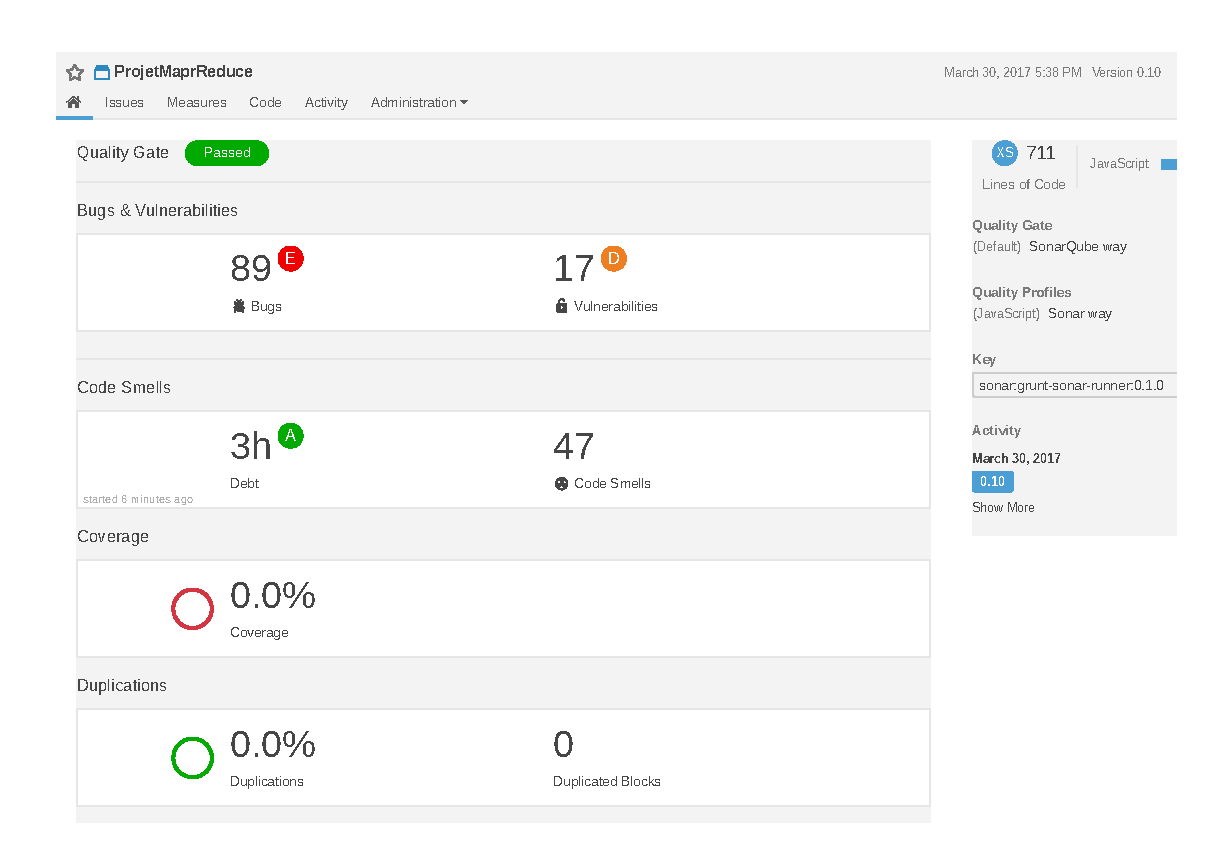
\includegraphics[scale=0.7]{images/sonarqube.pdf}
        \caption{Résultats de SonarQube}
\end{figure}

Nous remarquons que 83 bugs est un nombre assez importants et cela peut être amélioré. Aussi, il y a 17 vulnérabilités dûes principalement aux {\bf console.log} rencontrés dans les fonctions de tests unitaires et dans le résultat du mapReduce process. Nous laissons quand même ces console.log, même si déconseillé dans les projets, pour les besoins du client et des tests unitaires. Les failles de sécurité viennent aussi de l'utilisation de la fonction \emph{eval()} dont nous avons donné l'intérêt dans le chapitre d'Implémentation. Nous laissons quand même cette fonction parce que, dans le contexte de notre projet, il n'est pas très grave de l'utiliser surtout que le site est hébergé sur les serveurs du CREMI. \\
D'autre part, les résultats sont satisfaisants vis-à-vis de la duplication de code (un taux nul) et des heures de dettes techniques\footnote{Les dettes étant le temps qu'une entreprise aurait mis pour déboguer le code.}.\\

Après avoir revu le code en vue de correction de bugs, les nouveaux résultats obtenus par SonarQube sont ceux de la figure ci-dessous.


